\sisetup{locale = EN} 
\title{\textbf{\rmfamily Hadron Spectroscopy}}
\subtitle{Hadrons and their Properties}
\author[~\PersonHadrons~]{{\PersonHadrons}}
\institute[\WorkGroup]{ \University}
\date{\dateMC}
\usepackage{ccicons}

\tikzstyle{state}=[
    circle,
    minimum size =1.25cm
    draw=black,
    thick,
    fill=gray,
    text=white]

    
%%%%%%%%%%%%%%%%%%%%%%%%%%%%%%%%%%%%%%%%%%%%%%%%%%%%%%%%%%%%%%%%%%%%%%%%%%%%%%%%%%%%%%%%%%%%%%
%   Options for the footline
%%%%%%%%%%%%%%%%%%%%%%%%%%%%%%%%%%%%%%%%%%%%%%%%%%%%%%%%%%%%%%%%%%%%%%%%%%%%%%%%%%%%%%%%%%%%%%
\setbeamertemplate{footline}
{
\leavevmode%
\hbox{%
\begin{beamercolorbox}[wd=0.5\paperwidth,ht=2.25ex,dp=1ex,center]{author in foot}%
\usebeamerfont{author in foot} \parbox{0.5\paperwidth}{\insertsubsection{}}
\end{beamercolorbox}%
\begin{beamercolorbox}[wd=0.11\paperwidth,ht=2.25ex,dp=1ex,center]{title in head/foot}%
\usebeamerfont{title in head/foot}
\end{beamercolorbox}%
\begin{beamercolorbox}[wd=0.385\paperwidth,ht=2.25ex,dp=1ex,right]{date in head/foot}%
\usebeamerfont{date in head/foot}\insertsection{}\hfill
|~Slide \insertframenumber{} \hspace*{2ex}%/ \inserttotalframenumber\hspace*{2ex}
\end{beamercolorbox}}%
\vskip0pt%
}


\begin{document}\selectlanguage{english}
\begin{frame}[plain]
\begin{center}
    \begin{tabular}{ccc}
 \parbox{0.33\textwidth}{\LogoInsitute}    &
 ~~~~\parbox{0.33\textwidth}{\includegraphics[height=1cm]{Logos And Group/LHCb_Logo.png}}   &  \parbox{0.33\textwidth}{\LogoUniversity}\\
\end{tabular}
\end{center}
\maketitle
\end{frame}
\begin{frame}{Today's day}

\footnotesize

\texttt{TODO: Put your timetable in here.}

\end{frame}
%%%%%%%%%%%%%%%%%%%%%%%%%%%%%%%%%%%%%%%%%%%%%%%%%%%%%%%%%%%%%%%%%%%%%%%%%%%%%%%%%%%%%%%%%%%%%%
\section{Scale Analysis}
%%%%%%%%%%%%%%%%%%%%%%%%%%%%%%%%%%%%%%%%%%%%%%%%%%%%%%%%%%%%%%%%%%%%%%%%%%%%%%%%%%%%%%%%%%%%%%
\begin{frame}{Deconstruction}

    \hspace{1.0cm} Atom \hspace{0.7cm} Atomic nucleus \hspace{1.0cm} Nucleon \hspace{1cm} Quarks\\\vspace{1cm}
     \includegraphics[width=12.5cm]{Figures Lecture on Hadrons/Scale Atom_Quark_updown-approach.png}\\\vspace{1cm}
   \hspace{1.1cm} $10^{-10}$\,m \hspace{1.2cm}  $10^{-14}$\,m  \hspace{1.5cm}  $10^{-15}$\,m  \hspace{1.3cm}  $<10^{-18}$\,m

\end{frame}
%%%%%%%%%%%%%%%%%%%%%%%%%%%%%%%%%%%%%%%%%%%%%%%%%%%%%%%%%%%%%%%%%%%%%%%%%%%%%%%%%%%%%%%%%%%%%%
\begin{frame}{Reconstruction}
     \hspace{1.0cm} Atom \hspace{0.7cm} Atomic nucleus \hspace{1.0cm} \textbf{\textcolor{red}{Hadrons}} \hspace{1cm} Quarks\\\vspace{1cm}
     \includegraphics[width=12.5cm]{Figures Lecture on Hadrons/Scale Atom_Quark_downup-approach.png}\\\vspace{1cm}
   \hspace{1.1cm} $10^{-10}$\,m \hspace{1.2cm}  $10^{-14}$\,m  \hspace{1.5cm}  $10^{-15}$\,m  \hspace{1.3cm}  $<10^{-18}$\,m
\end{frame}
%%%%%%%%%%%%%%%%%%%%%%%%%%%%%%%%%%%%%%%%%%%%%%%%%%%%%%%%%%%%%%%%%%%%%%%%%%%%%%%%%%%%%%%%%%%%%%
\section{Hadrons}

%%%%%%%%%%%%%%%%%%%%%%%%%%%%%%%%%%%%%%%%%%%%%%%%%%%%%%%%%%%%%%%%%%%%%%%%%%%%%%%%%%%%%%%%%%%%%%
\begin{frame}{How do you build Particles?}
    \centering
    \includegraphics[width=7cm]{Figures Lecture on Hadrons/Scale Atom_Quark_downup-approach_Hadron.png}
\begin{itemize}
    \item Under what conditions do quarks stick together to form particles?
    \item Can matter bind with antimatter? %\pause
    \item[\ding{43}] Your turn!
\end{itemize}
\end{frame}

%%%%%%%%%%%%%%%%%%%%%%%%%%%%%%%%%%%%%%%%%%%%%%%%%%%%%%%%%%%%%%%%%%%%%%%%%%%%%%%%%%%%%%%%%%%%%%
\newcommand\squareF{\raisebox{-2mm}{\scalebox{3}{\ding{110}}}}
\begin{frame}{LHCb Quark-Puzzle}
\textbf{Task:}\\ Build closed particles from quarks and antiquarks. \\ \begin{itemize}
    \item What are they called and under what conditions do quarks stick together to form a particle?
    \item Are there any peculiarities? %\pause
    \end{itemize}\\
\vspace{1cm}
\textbf{Write on the worksheet!}
\end{frame}
%%%%%%%%%%%%%%%%%%%%%%%%%%%%%%%%%%%%%%%%%%%%%%%%%%%%%%%%%%%%%%%%%%%%%%%%%%%%%%%%%%%%%%%%%%%%%%
\section{Properties of Hadrons}
%%%%%%%%%%%%%%%%%%%%%%%%%%%%%%%%%%%%%%%%%%%%%%%%%%%%%%%%%%%%%%%%%%%%%%%%%%%%%%%%%%%%%%%%%%%%%%
\begin{frame}{Hadrons I}
     \hspace{0.2cm} \textbf{How many quarks can be used to build stable particles?} \\
    \end{frame}
 %%%%%%%%%%%%%%%%%%%%%%%%%%%%%%%%%%%%%%%%%%%%%%%%%%%%%%%%%%%%%%%%%%%%%%%%%%%%%%%%%%%%%%%%%%%%%%
 \begin{frame}{Hadrons II}
\textbf{How many quarks can be used to build stable particles?}
\begin{table}[]
    \centering
    \begin{tabular}{ccc}
        \includegraphics[width=3cm]{Figures Lecture on Hadrons/QuarkPuzzle_Baryon.jpg}&\includegraphics[width=3cm]{Figures Lecture on Hadrons/QuarkPuzzle_Antibaryon.jpg}&\includegraphics[width=3cm]{Figures Lecture on Hadrons/QuarkPuzzle_Meson.jpg} \\
        &&\\
        Baryon &   Antibaryon  & Meson    \\
        $qqq$ &  $\Bar{q}\Bar{q}\Bar{q} $&$ q\Bar{q}$ \\
        &&\\
         \includegraphics[width=2.5cm]{Figures Lecture on Hadrons/Baryon_scheme.png} &\includegraphics[width=2.5cm]{Figures Lecture on Hadrons/Antibaryon_scheme.png} &\includegraphics[width=2.5cm]{Figures Lecture on Hadrons/Meson_scheme.png} 
    \end{tabular}
    \label{tab:my_label}
\end{table}
  \end{frame}

%%%%%%%%%%%%%%%%%%%%%%%%%%%%%%%%%%%%%%%%%%%%%%%%%%%%%%%%%%%%%%%%%%%%%%%%%%%%%%%%%%%%%%%%%%%%%%
\begin{frame}
\textbf{What colours then must quarks have? }\\ \textbf{Why are quarks coloured?}
\end{frame}


%%%%%%%%%%%%%%%%%%%%%%%%%%%%%%%%%%%%%%%%%%%%%%%%%%%%%%%%%%%%%%%%%%%%%%%%%%%%%%%%%%%%%%%%%%%%%%
\begin{frame}{Colour Charges}
    \begin{column}{.58\textwidth}
\\ \includegraphics[width=6cm]{Figures Introductory Lecture/Standard Model/BlackAdditiveColours.png}
\end{column}%
\begin{column}{.42\textwidth}

\begin{align*}
    \ket{\textmd{Baryons}}=\rotatebox[]{90}{\rightarrow}+\rotatebox[]{225}{\rightarrow}+\rotatebox[]{315}{\rightarrow}=\Vec{0}\\ 
    \ket{\textmd{Mesons}}=
    \begin{cases} \,\rotatebox[]{90}{\rightarrow}~+~\rotatebox[]{270}{\rightarrow}~=\Vec{0}\\
    \rotatebox[]{135}{\rightarrow}+\rotatebox[]{315}{\rightarrow}=\Vec{0}\\
    \rotatebox[]{225}{\rightarrow}+\rotatebox[]{45}{\rightarrow}=\Vec{0}
    \end{cases} 
\end{align*} %\pause
 \tcbox[tcbox raise base]{\parbox{3cm}{Hadrons are colour-neutral.}}\\ %\pause

 $\cdots$ and why do we define colour?
 \end{column}
 \end{frame}
 %%%%%%%%%%%%%%%%%%%%%%%%%%%%%%%%%%%%%%%%%%%%%%%%%%%%%%%%%%%%%%%%%%%%%%%%%%%%%%%%%%%%%%%%%%%%%%

%%%%%%%%%%%%%%%%%%%%%%%%%%%%%%%%%%%%%%%%%%%%%%%%%%%%%%%%%%%%%%%%%%%%%%%%%%%%%%%%%%%%%%%%%%%%%%
%%%%%%%%%%%%%%%%%%%%%%%%%%%%%%%%%%%%%%%%%%%%%%%%%%%%%%%%%%%%%%%%%%%%%%%%%%%%%%%%%%%%%%%%%%%%%%
\begin{frame}{Can we observe individual quarks?}

            \def\d{1.25}
            \def\R{0.5}
            \def\N{{1.25*(\R+\d)}}
            \def\T{{1.75*(\R+\d)}}
\begin{tikzpicture}
\begin{feynman}[nodes=circle]
\vertex (a1){u};
    \vertex[below= 0.5cm of a1] (a1M);

    \vertex[right= 2cm of a1M](a2) {\,};
        \vertex[below= 0.5cm of a2] (a2M);
        \vertex[right= 2cm of a2M](a3) {\,};
            \vertex[below= 0.5cm of a3] (a3M);
    \vertex[right= 2cm of a3M](a4) {\,};
    \vertex[above=1.1cm of a1] (b1) {\,};
        \vertex[above= 0.5cm of b1] (b1M);
    \vertex[right= 2cm of b1M](b2) {\,};
        \vertex[above= 0.5cm of b2] (b2M);
    \vertex[right= 2cm of b2M](b3) {\,};
     \vertex[above= 0.5cm of b3] (b3M);
  \vertex[right = 2cm of b3M](b4) {\,};
  \vertex[below= 0.5cm of a4] (a4M);
  \vertex[above= 0.5cm of b4] (b4M);


        \vertex[below= 0.5cm of a1M] (a1MM);
        \vertex[below= 0.5cm of a2M] (a2MM);
        \vertex[below= 0.5cm of a3M] (a3MM);
        \vertex[above= 0.5cm of b1M] (b1MM);
        \vertex[above= 0.5cm of b2M] (b2MM);
        \vertex[above= 0.5cm of b3M] (b3MM);
        


        \vertex[right = 0.5cm of b1](b1r);
        \vertex[right = 0.5cm of b2](b2r);
        \vertex[right = 0.5cm of b3](b3r);
        \vertex[right = 0.5cm of a1](a1r);
        \vertex[right = 0.5cm of a2](a2r);
        \vertex[right = 0.5cm of a3](a3r);

        \vertex[left = 0.5cm of b1](b1l);
        \vertex[left = 0.5cm of b2](b2l);
        \vertex[left = 0.5cm of b3](b3l);
         \vertex[left = 0.5cm of a1](a1l);
        \vertex[left = 0.5cm of a2](a2l);
        \vertex[left = 0.5cm of a3](a3l);
  
        \vertex[above=1.2cm of a4] (a4n);
        \vertex[above=0.8cm of a4] (a4nn);
        \vertex[below=1.2cm of b4] (b4n);
        \vertex[below=0.8cm of b4] (b4nn);

        \vertex[right = 0.5cm of b4](b4r);          
        \vertex[right = 0.5cm of b4](b4r);
        \vertex[right = 0.5cm of a4](a4r);
        \vertex[left = 0.5cm of a4](a4l); 
        \vertex[left = 0.5cm of b4](b4l);
        
        \vertex[right = 0.5cm of b4n](b4nr);
        \vertex[right = 0.5cm of a4n](a4nr);
        \vertex[left = 0.5cm of a4n](a4nl); 
        \vertex[left = 0.5cm of b4n](b4nl);
        \vertex[above = 0.5cm of a4n](a4nM);
        \vertex[below = 0.5cm of b4n](b4nM);

        \vertex[above= 1.55cm of a3] (m3);
        \vertex[right= .1cm of m3] (m3l);

   

\draw[white, inner color= blue, outer color=white,]                      (a1) circle (\R) node  {\LARGE\textbf{\textcolor{white}{{\textmd{d}}}}};
\draw[white, inner color= yellow, outer color=white,]                      (b1) circle (\R) node  {\LARGE\textbf{\textcolor{black}{$\Bar{\textmd{s}}$}}};
    \diagram* {
 (a1) -- [gluon, thick, edge label=$g$] (b1),
  (a1M) -> [thick, edge label'=$\Vec{F}$,opacity=0] (a1MM),
   (b1M) -> [thick, edge label=$\Vec{F}$,opacity=0] (b1MM),
    (a3M) -> [thick, edge label'=$\Vec{F}$,opacity=0] (a3MM),
   (b3M) -> [thick, edge label=$\Vec{F}$,opacity=0] (b3MM),
    (a1M) -- [quarter right] (a1r) -- [] (b1r) -- [quarter right] (b1M) -- [quarter right] (b1l) -- [edge label'=\rotatebox{+90}{Meson}] (a1l)-- [quarter right] (a1M),   
        };
       %CONFINEMENT GRAFIK 
  \end{feynman}

\end{tikzpicture} \\
  We are building such a meson.
\end{frame}

\begin{frame}{Confinement}
%CONFINEMENT GRAFIK 
            \def\d{1.25}
            \def\R{0.5}
            \def\N{{1.25*(\R+\d)}}
            \def\T{{1.75*(\R+\d)}}
\begin{tikzpicture}
\begin{feynman}[nodes=circle]
\vertex (a1){u};
    \vertex[below= 0.5cm of a1] (a1M);

    \vertex[right= 2cm of a1M](a2) {\,};
        \vertex[below= 0.5cm of a2] (a2M);
        \vertex[right= 2cm of a2M](a3) {\,};
            \vertex[below= 0.5cm of a3] (a3M);
    \vertex[right= 2cm of a3M](a4) {\,};
    \vertex[above=1.1cm of a1] (b1) {\,};
        \vertex[above= 0.5cm of b1] (b1M);
    \vertex[right= 2cm of b1M](b2) {\,};
        \vertex[above= 0.5cm of b2] (b2M);
    \vertex[right= 2cm of b2M](b3) {\,};
     \vertex[above= 0.5cm of b3] (b3M);
  \vertex[right = 2cm of b3M](b4) {\,};
  \vertex[below= 0.5cm of a4] (a4M);
  \vertex[above= 0.5cm of b4] (b4M);


        \vertex[below= 0.5cm of a1M] (a1MM);
        \vertex[below= 0.5cm of a2M] (a2MM);
        \vertex[below= 0.5cm of a3M] (a3MM);
        \vertex[above= 0.5cm of b1M] (b1MM);
        \vertex[above= 0.5cm of b2M] (b2MM);
        \vertex[above= 0.5cm of b3M] (b3MM);
        


        \vertex[right = 0.5cm of b1](b1r);
        \vertex[right = 0.5cm of b2](b2r);
        \vertex[right = 0.5cm of b3](b3r);
        \vertex[right = 0.5cm of a1](a1r);
        \vertex[right = 0.5cm of a2](a2r);
        \vertex[right = 0.5cm of a3](a3r);

        \vertex[left = 0.5cm of b1](b1l);
        \vertex[left = 0.5cm of b2](b2l);
        \vertex[left = 0.5cm of b3](b3l);
         \vertex[left = 0.5cm of a1](a1l);
        \vertex[left = 0.5cm of a2](a2l);
        \vertex[left = 0.5cm of a3](a3l);
  
        \vertex[above=1.2cm of a4] (a4n);
        \vertex[above=0.8cm of a4] (a4nn);
        \vertex[below=1.2cm of b4] (b4n);
        \vertex[below=0.8cm of b4] (b4nn);

        \vertex[right = 0.5cm of b4](b4r);          
        \vertex[right = 0.5cm of b4](b4r);
        \vertex[right = 0.5cm of a4](a4r);
        \vertex[left = 0.5cm of a4](a4l); 
        \vertex[left = 0.5cm of b4](b4l);
        
        \vertex[right = 0.5cm of b4n](b4nr);
        \vertex[right = 0.5cm of a4n](a4nr);
        \vertex[left = 0.5cm of a4n](a4nl); 
        \vertex[left = 0.5cm of b4n](b4nl);
        \vertex[above = 0.5cm of a4n](a4nM);
        \vertex[below = 0.5cm of b4n](b4nM);

        \vertex[above= 1.55cm of a3] (m3);
        \vertex[right= .1cm of m3] (m3l);

   
%\draw[white, inner color= blue, outer color=white,]                      (a4) circle (\R) node  {\LARGE\textbf{\textcolor{white}{$\Bar{\textmd{u}}$}}};

\draw[white, inner color= blue, outer color=white,]                      (a1) circle (\R) node  {\LARGE\textbf{\textcolor{white}{{\textmd{d}}}}};
% \draw[white, inner color= blue, outer color=white,]                      (a2) circle (\R) node  {\LARGE\textbf{\textcolor{white}{{\textmd{d}}}}};
% \draw[white, inner color= blue, outer color=white,]                      (a3) circle (\R) node  {\LARGE\textbf{\textcolor{white}{{\textmd{d}}}}};
% \draw[white, inner color= blue, outer color=white,]                      (a4) circle (\R) node  {\LARGE\textbf{\textcolor{white}{{\textmd{d}}}}};
% \draw[white, inner color= yellow, outer color=white,]                      (a4n) circle (\R) node  {\LARGE\textbf{\textcolor{black}{$\Bar{\textmd{u}}$}}};
\draw[white, inner color= yellow, outer color=white,]                      (b1) circle (\R) node  {\LARGE\textbf{\textcolor{black}{$\Bar{\textmd{s}}$}}};
% \draw[white, inner color= yellow, outer color=white,]                      (b2) circle (\R) node  {\LARGE\textbf{\textcolor{black}{$\Bar{\textmd{s}}$}}};
% \draw[white, inner color= yellow, outer color=white,]                      (b3) circle (\R) node  {\LARGE\textbf{\textcolor{black}{$\Bar{\textmd{s}}$}}};
% \draw[white, inner color= yellow, outer color=white,]                      (b4) circle (\R) node  {\LARGE\textbf{\textcolor{black}{$\Bar{\textmd{s}}$}}};
% \draw[white, inner color= blue, outer color=white,]                      (b4n) circle (\R) node  {\LARGE\textbf{\textcolor{white}{{\textmd{u}}}}};
    \diagram* {
 (a1) -- [gluon, thick, edge label=$g$] (b1),
  % (b4nn) -- [gluon, thick, edge label=$g$] (b4),
  % (a4) -- [gluon, thick, edge label=$g$] (a4nn),
  (a1M) -> [thick, edge label'=$\Vec{F}$] (a1MM),
   (b1M) -> [thick, edge label=$\Vec{F}$] (b1MM),
 %   (a2M) -> [thick, edge label'=$\Vec{F}$] (a2MM),
 %  (b2M) -> [thick, edge label=$\Vec{F}$] (b2MM),
    (a3M) -> [thick, edge label'=$\Vec{F}$,opacity=0] (a3MM),
   (b3M) -> [thick, edge label=$\Vec{F}$,opacity=0] (b3MM),
% (a2) -- [gluon, thick, edge label=$g$] (b2),
% (a3) -- [gluon, thick, edge label=$g$] (b3),
%(m3) -- [] (m3l),
% (m3l) -- [gluon,thick,quarter left, edge label=$g$] (b4nl),
% (m3l) -- [gluon,thick, quarter right, edge label=$g$] (a4nl),
 % (a4nl)-- [fermion, thick, in=-90, out=-180,opacity=0] (m3l),
 % (m3l)-- [fermion, thick, in=-180, out=90,opacity=0] (b4nl),

    (a1M) -- [quarter right] (a1r) -- [] (b1r) -- [quarter right] (b1M) -- [quarter right] (b1l) -- [edge label'=\rotatebox{+90}{Meson}] (a1l)-- [quarter right] (a1M),
    % (a2M) -- [quarter right] (a2r) -- [] (b2r) -- [quarter right] (b2M) -- [quarter right] (b2l) -- [] (a2l)-- [quarter right] (a2M),
    % (a3M) -- [quarter right] (a3r) -- [] (b3r) -- [quarter right] (b3M) -- [quarter right] (b3l) -- [] (a3l)-- [quarter right] (a3M),
    %  (a4M) -- [quarter right] (a4r) -- [] (a4nr) -- [quarter right] (a4nM) -- [quarter right] (a4nl) -- [] (a4l)-- [quarter right] (a4M),
    %  (b4M) -- [quarter left] (b4r) -- [] (b4nr) -- [quarter left] (b4nM) -- [quarter left] (b4nl) -- [] (b4l)-- [quarter left] (b4M),
   
        };
       %CONFINEMENT GRAFIK 
  \end{feynman}
  
\end{tikzpicture} \\
A meson is pulled.
\end{frame}
%%%%%%%%%%%%%%%%%%%%%%%%%%%%%%%%%%%%%%%%%%%%%%%%%%%%%%%%%%%%%%%%%%%%%%%%%%%%%%%%%%%%%%%%%%%%%%
\begin{frame}{Confinement}\addtocounter{framenumber}{-1}
%CONFINEMENT GRAFIK 
            \def\d{1.25}
            \def\R{0.5}
            \def\N{{1.25*(\R+\d)}}
            \def\T{{1.75*(\R+\d)}}
\begin{tikzpicture}
\begin{feynman}[nodes=circle]
\vertex (a1){u};
    \vertex[below= 0.5cm of a1] (a1M);

    \vertex[right= 2cm of a1M](a2) {\,};
        \vertex[below= 0.5cm of a2] (a2M);
        \vertex[right= 2cm of a2M](a3) {\,};
            \vertex[below= 0.5cm of a3] (a3M);
    \vertex[right= 2cm of a3M](a4) {\,};
    \vertex[above=1.1cm of a1] (b1) {\,};
        \vertex[above= 0.5cm of b1] (b1M);
    \vertex[right= 2cm of b1M](b2) {\,};
        \vertex[above= 0.5cm of b2] (b2M);
    \vertex[right= 2cm of b2M](b3) {\,};
     \vertex[above= 0.5cm of b3] (b3M);
  \vertex[right = 2cm of b3M](b4) {\,};
  \vertex[below= 0.5cm of a4] (a4M);
  \vertex[above= 0.5cm of b4] (b4M);


        \vertex[below= 0.5cm of a1M] (a1MM);
        \vertex[below= 0.5cm of a2M] (a2MM);
        \vertex[below= 0.5cm of a3M] (a3MM);
        \vertex[above= 0.5cm of b1M] (b1MM);
        \vertex[above= 0.5cm of b2M] (b2MM);
        \vertex[above= 0.5cm of b3M] (b3MM);
        


        \vertex[right = 0.5cm of b1](b1r);
        \vertex[right = 0.5cm of b2](b2r);
        \vertex[right = 0.5cm of b3](b3r);
        \vertex[right = 0.5cm of a1](a1r);
        \vertex[right = 0.5cm of a2](a2r);
        \vertex[right = 0.5cm of a3](a3r);

        \vertex[left = 0.5cm of b1](b1l);
        \vertex[left = 0.5cm of b2](b2l);
        \vertex[left = 0.5cm of b3](b3l);
         \vertex[left = 0.5cm of a1](a1l);
        \vertex[left = 0.5cm of a2](a2l);
        \vertex[left = 0.5cm of a3](a3l);
  
        \vertex[above=1.2cm of a4] (a4n);
        \vertex[above=0.8cm of a4] (a4nn);
        \vertex[below=1.2cm of b4] (b4n);
        \vertex[below=0.8cm of b4] (b4nn);

        \vertex[right = 0.5cm of b4](b4r);          
        \vertex[right = 0.5cm of b4](b4r);
        \vertex[right = 0.5cm of a4](a4r);
        \vertex[left = 0.5cm of a4](a4l); 
        \vertex[left = 0.5cm of b4](b4l);
        
        \vertex[right = 0.5cm of b4n](b4nr);
        \vertex[right = 0.5cm of a4n](a4nr);
        \vertex[left = 0.5cm of a4n](a4nl); 
        \vertex[left = 0.5cm of b4n](b4nl);
        \vertex[above = 0.5cm of a4n](a4nM);
        \vertex[below = 0.5cm of b4n](b4nM);

        \vertex[above= 1.55cm of a3] (m3);
        \vertex[right= .1cm of m3] (m3l);

   
%\draw[white, inner color= blue, outer color=white,]                      (a4) circle (\R) node  {\LARGE\textbf{\textcolor{white}{$\Bar{\textmd{u}}$}}};

\draw[white, inner color= blue, outer color=white,]                      (a1) circle (\R) node  {\LARGE\textbf{\textcolor{white}{{\textmd{d}}}}};
\draw[white, inner color= blue, outer color=white,]                      (a2) circle (\R) node  {\LARGE\textbf{\textcolor{white}{{\textmd{d}}}}};
\draw[white, inner color= blue, outer color=white,]                      (a3) circle (\R) node  {\LARGE\textbf{\textcolor{white}{{\textmd{d}}}}};
% \draw[white, inner color= blue, outer color=white,]                      (a4) circle (\R) node  {\LARGE\textbf{\textcolor{white}{{\textmd{d}}}}};
% \draw[white, inner color= yellow, outer color=white,]                      (a4n) circle (\R) node  {\LARGE\textbf{\textcolor{black}{$\Bar{\textmd{u}}$}}};
\draw[white, inner color= yellow, outer color=white,]                      (b1) circle (\R) node  {\LARGE\textbf{\textcolor{black}{$\Bar{\textmd{s}}$}}};
\draw[white, inner color= yellow, outer color=white,]                      (b2) circle (\R) node  {\LARGE\textbf{\textcolor{black}{$\Bar{\textmd{s}}$}}};
\draw[white, inner color= yellow, outer color=white,]                      (b3) circle (\R) node  {\LARGE\textbf{\textcolor{black}{$\Bar{\textmd{s}}$}}};
% \draw[white, inner color= yellow, outer color=white,]                      (b4) circle (\R) node  {\LARGE\textbf{\textcolor{black}{$\Bar{\textmd{s}}$}}};
% \draw[white, inner color= blue, outer color=white,]                      (b4n) circle (\R) node  {\LARGE\textbf{\textcolor{white}{{\textmd{u}}}}};
    \diagram* {
 (a1) -- [gluon, thick, edge label=$g$] (b1),
 % (b4nn) -- [gluon, thick, edge label=$g$] (b4),
 % (a4) -- [gluon, thick, edge label=$g$] (a4nn),
 (a1M) -> [thick, edge label'=$\Vec{F}$] (a1MM),
  (b1M) -> [thick, edge label=$\Vec{F}$] (b1MM),
   (a2M) -> [thick, edge label'=$\Vec{F}$] (a2MM),
  (b2M) -> [thick, edge label=$\Vec{F}$] (b2MM),
   (a3M) -> [thick, edge label'=$\Vec{F}$] (a3MM),
  (b3M) -> [thick, edge label=$\Vec{F}$] (b3MM),
(a2) -- [gluon, thick, edge label=$g$] (b2),
(a3) -- [gluon, thick, edge label=$g$] (b3),
%(m3) -- [] (m3l),
% (m3l) -- [gluon,thick,quarter left, edge label=$g$] (b4nl),
% (m3l) -- [gluon,thick, quarter right, edge label=$g$] (a4nl),
% (a4nl)-- [fermion, thick, in=-90, out=-180] (m3l),
% (m3l)-- [fermion, thick, in=-180, out=90] (b4nl),

    (a1M) -- [quarter right] (a1r) -- [] (b1r) -- [quarter right] (b1M) -- [quarter right] (b1l) -- [edge label'=\rotatebox{+90}{Meson}] (a1l)-- [quarter right] (a1M),
    (a2M) -- [quarter right] (a2r) -- [] (b2r) -- [quarter right] (b2M) -- [quarter right] (b2l) -- [] (a2l)-- [quarter right] (a2M),
    (a3M) -- [quarter right] (a3r) -- [] (b3r) -- [quarter right] (b3M) -- [quarter right] (b3l) -- [] (a3l)-- [quarter right] (a3M),
     % (a4M) -- [quarter right] (a4r) -- [] (a4nr) -- [quarter right] (a4nM) -- [quarter right] (a4nl) -- [] (a4l)-- [quarter right] (a4M),
     % (b4M) -- [quarter left] (b4r) -- [] (b4nr) -- [quarter left] (b4nM) -- [quarter left] (b4nl) -- [] (b4l)-- [quarter left] (b4M),
   
        };
       %CONFINEMENT GRAFIK 
  \end{feynman}
\end{tikzpicture} \\
A meson is pulled, when does it fly apart?
\end{frame}
%%%%%%%%%%%%%%%%%%%%%%%%%%%%%%%%%%%%%%%%%%%%%%%%%%%%%%%%%%%%%%%%%%%%%%%%%%%%%%%%%%%%%%%%%%%%%%
\begin{frame}{Confinement}\addtocounter{framenumber}{-1}
%CONFINEMENT GRAFIK 
            \def\d{1.25}
            \def\R{0.5}
            \def\N{{1.25*(\R+\d)}}
            \def\T{{1.75*(\R+\d)}}
\begin{tikzpicture}
\begin{feynman}[nodes=circle]
\vertex (a1){u};
    \vertex[below= 0.5cm of a1] (a1M);

    \vertex[right= 2cm of a1M](a2) {\,};
        \vertex[below= 0.5cm of a2] (a2M);
        \vertex[right= 2cm of a2M](a3) {\,};
            \vertex[below= 0.5cm of a3] (a3M);
    \vertex[right= 2cm of a3M](a4) {\,};
    \vertex[above=1.1cm of a1] (b1) {\,};
        \vertex[above= 0.5cm of b1] (b1M);
    \vertex[right= 2cm of b1M](b2) {\,};
        \vertex[above= 0.5cm of b2] (b2M);
    \vertex[right= 2cm of b2M](b3) {\,};
     \vertex[above= 0.5cm of b3] (b3M);
  \vertex[right = 2cm of b3M](b4) {\,};
  \vertex[below= 0.5cm of a4] (a4M);
  \vertex[above= 0.5cm of b4] (b4M);


        \vertex[below= 0.5cm of a1M] (a1MM);
        \vertex[below= 0.5cm of a2M] (a2MM);
        \vertex[below= 0.5cm of a3M] (a3MM);
        \vertex[above= 0.5cm of b1M] (b1MM);
        \vertex[above= 0.5cm of b2M] (b2MM);
        \vertex[above= 0.5cm of b3M] (b3MM);
        


        \vertex[right = 0.5cm of b1](b1r);
        \vertex[right = 0.5cm of b2](b2r);
        \vertex[right = 0.5cm of b3](b3r);
        \vertex[right = 0.5cm of a1](a1r);
        \vertex[right = 0.5cm of a2](a2r);
        \vertex[right = 0.5cm of a3](a3r);

        \vertex[left = 0.5cm of b1](b1l);
        \vertex[left = 0.5cm of b2](b2l);
        \vertex[left = 0.5cm of b3](b3l);
         \vertex[left = 0.5cm of a1](a1l);
        \vertex[left = 0.5cm of a2](a2l);
        \vertex[left = 0.5cm of a3](a3l);
  
        \vertex[above=1.2cm of a4] (a4n);
        \vertex[above=0.8cm of a4] (a4nn);
        \vertex[below=1.2cm of b4] (b4n);
        \vertex[below=0.8cm of b4] (b4nn);

        \vertex[right = 0.5cm of b4](b4r);          
        \vertex[right = 0.5cm of b4](b4r);
        \vertex[right = 0.5cm of a4](a4r);
        \vertex[left = 0.5cm of a4](a4l); 
        \vertex[left = 0.5cm of b4](b4l);
        
        \vertex[right = 0.5cm of b4n](b4nr);
        \vertex[right = 0.5cm of a4n](a4nr);
        \vertex[left = 0.5cm of a4n](a4nl); 
        \vertex[left = 0.5cm of b4n](b4nl);
        \vertex[above = 0.5cm of a4n](a4nM);
        \vertex[below = 0.5cm of b4n](b4nM);

        \vertex[above= 1.55cm of a3] (m3);
        \vertex[right= .1cm of m3] (m3l);

   
%\draw[white, inner color= blue, outer color=white,]                      (a4) circle (\R) node  {\LARGE\textbf{\textcolor{white}{$\Bar{\textmd{u}}$}}};

\draw[white, inner color= blue, outer color=white,]                      (a1) circle (\R) node  {\LARGE\textbf{\textcolor{white}{{\textmd{d}}}}};
\draw[white, inner color= blue, outer color=white,]                      (a2) circle (\R) node  {\LARGE\textbf{\textcolor{white}{{\textmd{d}}}}};
\draw[white, inner color= blue, outer color=white,]                      (a3) circle (\R) node  {\LARGE\textbf{\textcolor{white}{{\textmd{d}}}}};
% \draw[white, inner color= blue, outer color=white,]                      (a4) circle (\R) node  {\LARGE\textbf{\textcolor{white}{{\textmd{d}}}}};
\draw[white, inner color= yellow, outer color=white,]                      (a4n) circle (\R) node  {\LARGE\textbf{\textcolor{black}{$\Bar{\textmd{u}}$}}};
\draw[white, inner color= yellow, outer color=white,]                      (b1) circle (\R) node  {\LARGE\textbf{\textcolor{black}{$\Bar{\textmd{s}}$}}};
\draw[white, inner color= yellow, outer color=white,]                      (b2) circle (\R) node  {\LARGE\textbf{\textcolor{black}{$\Bar{\textmd{s}}$}}};
\draw[white, inner color= yellow, outer color=white,]                      (b3) circle (\R) node  {\LARGE\textbf{\textcolor{black}{$\Bar{\textmd{s}}$}}};
% \draw[white, inner color= yellow, outer color=white,]                      (b4) circle (\R) node  {\LARGE\textbf{\textcolor{black}{$\Bar{\textmd{s}}$}}};
 \draw[white, inner color= blue, outer color=white,]                      (b4n) circle (\R) node  {\LARGE\textbf{\textcolor{white}{{\textmd{u}}}}};
    \diagram* {
 (a1) -- [gluon, thick, edge label=$g$] (b1),
 % (b4nn) -- [gluon, thick, edge label=$g$] (b4),
 % (a4) -- [gluon, thick, edge label=$g$] (a4nn),
 (a1M) -> [thick, edge label'=$\Vec{F}$] (a1MM),
  (b1M) -> [thick, edge label=$\Vec{F}$] (b1MM),
   (a2M) -> [thick, edge label'=$\Vec{F}$] (a2MM),
  (b2M) -> [thick, edge label=$\Vec{F}$] (b2MM),
   (a3M) -> [thick, edge label'=$\Vec{F}$] (a3MM),
  (b3M) -> [thick, edge label=$\Vec{F}$] (b3MM),
(a2) -- [gluon, thick, edge label=$g$] (b2),
(a3) -- [gluon, thick, edge label=$g$] (b3),
%(m3) -- [] (m3l),
% (m3l) -- [gluon,thick,quarter left, edge label=$g$] (b4nl),
% (m3l) -- [gluon,thick, quarter right, edge label=$g$] (a4nl),
(a4nl)-- [fermion, thick, in=-90, out=-180] (m3l),
(m3l)-- [fermion, thick, in=-180, out=90] (b4nl),

    (a1M) -- [quarter right] (a1r) -- [] (b1r) -- [quarter right] (b1M) -- [quarter right] (b1l) -- [edge label'=\rotatebox{+90}{Meson}] (a1l)-- [quarter right] (a1M),
    (a2M) -- [quarter right] (a2r) -- [] (b2r) -- [quarter right] (b2M) -- [quarter right] (b2l) -- [] (a2l)-- [quarter right] (a2M),
    (a3M) -- [quarter right] (a3r) -- [] (b3r) -- [quarter right] (b3M) -- [quarter right] (b3l) -- [] (a3l)-- [quarter right] (a3M),
     % (a4M) -- [quarter right] (a4r) -- [] (a4nr) -- [quarter right] (a4nM) -- [quarter right] (a4nl) -- [] (a4l)-- [quarter right] (a4M),
     % (b4M) -- [quarter left] (b4r) -- [] (b4nr) -- [quarter left] (b4nM) -- [quarter left] (b4nl) -- [] (b4l)-- [quarter left] (b4M),
   
        };
       %CONFINEMENT GRAFIK 
  \end{feynman}
\end{tikzpicture} \\
The energy of the strong field forms a u$\Bar{\textmd{u}}$ pair.
\end{frame}
%%%%%%%%%%%%%%%%%%%%%%%%%%%%%%%%%%%%%%%%%%%%%%%%%%%%%%%%%%%%%%%%%%%%%%%%%%%%%%%%%%%%%%%%%%%%%%
\begin{frame}{Confinement}\addtocounter{framenumber}{-1}
%CONFINEMENT GRAFIK 
            \def\d{1.25}
            \def\R{0.5}
            \def\N{{1.25*(\R+\d)}}
            \def\T{{1.75*(\R+\d)}}
\begin{tikzpicture}
\begin{feynman}[nodes=circle]
\vertex (a1){u};
    \vertex[below= 0.5cm of a1] (a1M);

    \vertex[right= 2cm of a1M](a2) {\,};
        \vertex[below= 0.5cm of a2] (a2M);
        \vertex[right= 2cm of a2M](a3) {\,};
            \vertex[below= 0.5cm of a3] (a3M);
    \vertex[right= 2cm of a3M](a4) {\,};
    \vertex[above=1.1cm of a1] (b1) {\,};
        \vertex[above= 0.5cm of b1] (b1M);
    \vertex[right= 2cm of b1M](b2) {\,};
        \vertex[above= 0.5cm of b2] (b2M);
    \vertex[right= 2cm of b2M](b3) {\,};
     \vertex[above= 0.5cm of b3] (b3M);
  \vertex[right = 2cm of b3M](b4) {\,};
  \vertex[below= 0.5cm of a4] (a4M);
  \vertex[above= 0.5cm of b4] (b4M);


        \vertex[below= 0.5cm of a1M] (a1MM);
        \vertex[below= 0.5cm of a2M] (a2MM);
        \vertex[below= 0.5cm of a3M] (a3MM);
        \vertex[above= 0.5cm of b1M] (b1MM);
        \vertex[above= 0.5cm of b2M] (b2MM);
        \vertex[above= 0.5cm of b3M] (b3MM);
        


        \vertex[right = 0.5cm of b1](b1r);
        \vertex[right = 0.5cm of b2](b2r);
        \vertex[right = 0.5cm of b3](b3r);
        \vertex[right = 0.5cm of a1](a1r);
        \vertex[right = 0.5cm of a2](a2r);
        \vertex[right = 0.5cm of a3](a3r);

        \vertex[left = 0.5cm of b1](b1l);
        \vertex[left = 0.5cm of b2](b2l);
        \vertex[left = 0.5cm of b3](b3l);
         \vertex[left = 0.5cm of a1](a1l);
        \vertex[left = 0.5cm of a2](a2l);
        \vertex[left = 0.5cm of a3](a3l);
  
        \vertex[above=1.2cm of a4] (a4n);
        \vertex[above=0.8cm of a4] (a4nn);
        \vertex[below=1.2cm of b4] (b4n);
        \vertex[below=0.8cm of b4] (b4nn);

        \vertex[right = 0.5cm of b4](b4r);          
        \vertex[right = 0.5cm of b4](b4r);
        \vertex[right = 0.5cm of a4](a4r);
        \vertex[left = 0.5cm of a4](a4l); 
        \vertex[left = 0.5cm of b4](b4l);
        
        \vertex[right = 0.5cm of b4n](b4nr);
        \vertex[right = 0.5cm of a4n](a4nr);
        \vertex[left = 0.5cm of a4n](a4nl); 
        \vertex[left = 0.5cm of b4n](b4nl);
        \vertex[above = 0.5cm of a4n](a4nM);
        \vertex[below = 0.5cm of b4n](b4nM);

        \vertex[above= 1.55cm of a3] (m3);
        \vertex[right= .1cm of m3] (m3l);

   
%\draw[white, inner color= blue, outer color=white,]                      (a4) circle (\R) node  {\LARGE\textbf{\textcolor{white}{$\Bar{\textmd{u}}$}}};

\draw[white, inner color= blue, outer color=white,]                      (a1) circle (\R) node  {\LARGE\textbf{\textcolor{white}{{\textmd{d}}}}};
\draw[white, inner color= blue, outer color=white,]                      (a2) circle (\R) node  {\LARGE\textbf{\textcolor{white}{{\textmd{d}}}}};
\draw[white, inner color= blue, outer color=white,]                      (a3) circle (\R) node  {\LARGE\textbf{\textcolor{white}{{\textmd{d}}}}};
\draw[white, inner color= blue, outer color=white,]                      (a4) circle (\R) node  {\LARGE\textbf{\textcolor{white}{{\textmd{d}}}}};
\draw[white, inner color= yellow, outer color=white,]                      (a4n) circle (\R) node  {\LARGE\textbf{\textcolor{black}{$\Bar{\textmd{u}}$}}};
\draw[white, inner color= yellow, outer color=white,]                      (b1) circle (\R) node  {\LARGE\textbf{\textcolor{black}{$\Bar{\textmd{s}}$}}};
\draw[white, inner color= yellow, outer color=white,]                      (b2) circle (\R) node  {\LARGE\textbf{\textcolor{black}{$\Bar{\textmd{s}}$}}};
\draw[white, inner color= yellow, outer color=white,]                      (b3) circle (\R) node  {\LARGE\textbf{\textcolor{black}{$\Bar{\textmd{s}}$}}};
\draw[white, inner color= yellow, outer color=white,]                      (b4) circle (\R) node  {\LARGE\textbf{\textcolor{black}{$\Bar{\textmd{s}}$}}};
\draw[white, inner color= blue, outer color=white,]                      (b4n) circle (\R) node  {\LARGE\textbf{\textcolor{white}{{\textmd{u}}}}};
    \diagram* {
 (a1) -- [gluon, thick, edge label=$g$] (b1),
 (b4nn) -- [gluon, thick, edge label=$g$] (b4),
 (a4) -- [gluon, thick, edge label=$g$] (a4nn),
 (a1M) -> [thick, edge label'=$\Vec{F}$] (a1MM),
  (b1M) -> [thick, edge label=$\Vec{F}$] (b1MM),
   (a2M) -> [thick, edge label'=$\Vec{F}$] (a2MM),
  (b2M) -> [thick, edge label=$\Vec{F}$] (b2MM),
   (a3M) -> [thick, edge label'=$\Vec{F}$] (a3MM),
  (b3M) -> [thick, edge label=$\Vec{F}$] (b3MM),
(a2) -- [gluon, thick, edge label=$g$] (b2),
(a3) -- [gluon, thick, edge label=$g$] (b3),
%(m3) -- [] (m3l),
% (m3l) -- [gluon,thick,quarter left, edge label=$g$] (b4nl),
% (m3l) -- [gluon,thick, quarter right, edge label=$g$] (a4nl),
(a4nl)-- [fermion, thick, in=-90, out=-180] (m3l),
(m3l)-- [fermion, thick, in=-180, out=90] (b4nl),

    (a1M) -- [quarter right] (a1r) -- [] (b1r) -- [quarter right] (b1M) -- [quarter right] (b1l) -- [edge label'=\rotatebox{+90}{Meson}] (a1l)-- [quarter right] (a1M),
    (a2M) -- [quarter right] (a2r) -- [] (b2r) -- [quarter right] (b2M) -- [quarter right] (b2l) -- [] (a2l)-- [quarter right] (a2M),
    (a3M) -- [quarter right] (a3r) -- [] (b3r) -- [quarter right] (b3M) -- [quarter right] (b3l) -- [] (a3l)-- [quarter right] (a3M),
     (a4M) -- [quarter right] (a4r) -- [] (a4nr) -- [quarter right] (a4nM) -- [quarter right] (a4nl) -- [] (a4l)-- [quarter right] (a4M),
     (b4M) -- [quarter left] (b4r) -- [] (b4nr) -- [quarter left] (b4nM) -- [quarter left] (b4nl) -- [] (b4l)-- [quarter left] (b4M),
   
        };
  \end{feynman}
\end{tikzpicture} \\
Quarks occur \underline{never} individually, hadrons are colour-neutral.
\end{frame}
%%%%%%%%%%%%%%%%%%%%%%%%%%%%%%%%%%%%%%%%%%%%%%%%%%%%%%%%%%%%%%%%%%%%%%%%%%%%%%%%%%%%%%%%%%%%%%
 \begin{frame}{Electrical Charges}
 \begin{center}
    What electrical charges can hadrons have? %\pause 
 \begin{spacing}{2.0}
     \begin{tabular}{rl}
 \T\B  Baryon   & $q_B/e\in\{-1, 0, 1, 2\}$ \\
 \T\B   Anti-Baryon   &$q_{\Bar{B}} /e\in\{-2, -1,0,1\}$ \\
 \T\B   Meson &$q_{M} /e\in\{-1,0,1\}$
 \end{tabular}
 \end{spacing}
 
\end{center}
 \end{frame}
%%%%%%%%%%%%%%%%%%%%%%%%%%%%%%%%%%%%%%%%%%%%%%%%%%%%%%%%%%%%%%%%%%%%%%%%%%%%%%%%%%%%%%%%%%%%%%
\begin{frame}
\textbf{Why doesn't the top quark bind?}
\end{frame}
\subsection{Picture: Airbus}
%%%%%%%%%%%%%%%%%%%%%%%%%%%%%%%%%%%%%%%%%%%%%%%%%%%%%%%%%%%%%%%%%%%%%%%%%%%%%%%%%%%%%%%%%%%%%%
\begin{frame}{Top-Quark}
It is:
    \[ m \propto \nicefrac{1}{\tau} \] %\pause
    \ding{43} Remember:

    \begin{table}[]
    \centering
    \begin{tabular}{ccc}
       \includegraphics[width=1.5cm]{Figures Lecture on Hadrons/SevenMountainsMilk.png}  &\parbox{4cm}{\vspace{-3cm}\begin{align*}m_{up}&= 2.2\,\textmd{MeV}/c^2 \\m_{top}&=174\,\textmd{GeV}/c^2 \end{align*}} & \includegraphics[width=3cm]{Figures Lecture on Hadrons/Airbus A321Neo.jpg}
       \end{tabular}  
\end{table} %\pause

\begin{center}
     \tcbox[tcbox raise base]{\parbox{7.2cm}{  A hadron with top flavour takes longer to form than the top quark decays.}}\\
   \end{center}
    \end{frame}
    \subsection{}
%%%%%%%%%%%%%%%%%%%%%%%%%%%%%%%%%%%%%%%%%%%%%%%%%%%%%%%%%%%%%%%%%%%%%%%%%%%%%%%%%%%%%%%%%%%%%%
\begin{frame}
\begin{minipage}{.3\textwidth}
\includegraphics[width=\textwidth]{Figures Lecture on Hadrons/Hadrons_Questionmark.png}
\end{minipage}
\begin{minipage}{.69\textwidth}
\hspace{-0.5cm}\textbf{How can hadrons be ordered?}
\end{minipage}
\end{frame}
%%%%%%%%%%%%%%%%%%%%%%%%%%%%%%%%%%%%%%%%%%%%%%%%%%%%%%%%%%%%%%%%%%%%%%%%%%%%%%%%%%%%%%%%%%%%%%

\begin{frame}{Sorting Scheme of Baryons}
\begin{center}
    

        \begin{tikzpicture}[yscale = 1.9]\footnotesize

    \draw[fill=LHCbLightBlue!80] (6,4.3)  to (4.9,4) to (3.8,4.2) to (6,4.3);
\draw[fill=LHCbLightBlue!80] (4.8,3) to (3.7,3.20) node[ below left] {$\Xi_{c}^{0}$} node [above right] {\scriptsize $dsc$}to (2.6,3.4) to(4.58,3.49) node [above] {\colorbox{white}{$\Sigma_{c}^{+}$}} node [below] {\scriptsize $udc$} to (7,3.6)  to(5.9,3.3) node [below right] {$\Xi_{c}^{+}$} node [above left=-3pt] {\colorbox{LHCbLightBlue!80}{\scriptsize $usc$}} to(4.8,3);
\draw[fill=LHCbLightBlue!80] (4.7,2) to (3.6,2.2) node [below left] {\colorbox{white}{$\Xi_{}^{-}$}} node [above right] {\scriptsize $dss$} to (2.5,2.4) node [below left] {\colorbox{white}{$\Sigma_{}^{-}$}} node [above right] {\scriptsize $dds$} to (1.4,2.6)to (3.6,2.7) node [above right] {$\Delta^0$} node [below] {\scriptsize $udd$} to(5.8,2.8) node [above] {$\Delta^+$} node [below] {\scriptsize $uud$} to  (8.0,2.9)to(6.9,2.6) node [below right] {\colorbox{white}{$\Sigma_{}^{+}$}} node [above left] {\scriptsize $uus$}  to(5.8,2.3) node [below right] {\colorbox{white}{$\Xi_{}^{0}$}} node [above=4pt] {\scriptsize $uss$} to(4.7,2);

        \node (ccc) at (5,5) {$\bullet$};
        
        \node (scc) at (4.9,4) {$\bullet$};
        \node (ucc) at (6,4.3) {$\bullet$};
        \node (dcc) at (3.8,4.2) {$\bullet$};
        
         \node (ssc) at (4.8,3) {$\bullet$};
         \node (dsc) at (3.7,3.20) {$\bullet$};
         \node (ddc) at (2.6,3.4) {$\bullet$};
             \node (usc) at (5.9,3.3) {$\bullet$};
             \node (uuc) at (7,3.6) {$\bullet$};

         
          \node (sss) at (4.7,2) {$\bullet$};
          \node (dss) at (3.6,2.2) {$\bullet$};
          \node (uds) at (4.63,2.53) {$\bullet$} ;
          \node (dds) at (2.5,2.4) {$\bullet$};    
          \node (ddd) at (1.4,2.6) {$\bullet$};
                    \node (uss) at (5.8,2.3) {$\bullet$};
                     \node (uus) at (6.9,2.6) {$\bullet$};
                     \node (uuu) at (8.0,2.9) {$\bullet$};

      \node (udc) at (4.58,3.49) {$\bullet$};
      \node (udd) at (3.6,2.7) {$\bullet$};
      \node (uud) at (5.8,2.8) {$\bullet$};



\draw[black, --] (5,5) node [above] {\colorbox{white}{$\Omega_{ccc}^{++}$}} to (4.9,4) node [below right] {$\Omega_{cc}^{+}$} node [above] {\colorbox{LHCbLightBlue!80}{\scriptsize $scc$}}   to (4.8,3) node [below left] {$\Omega_{c}^{0}$} node [above] {\colorbox{LHCbLightBlue!80}{\scriptsize $ssc$}}  to (4.7,2) node [below] {\colorbox{white}{$\Omega_{}^{-}$}} node [above=4pt] {\colorbox{LHCbLightBlue!80}{\scriptsize $sss$}} 

(5,5)to(6,4.3) node [above right] {\colorbox{white}{$\Xi_{cc}^{++}$}} node [ above left] {\scriptsize $ucc$~~~}  to(7,3.6) node [above right] {\colorbox{white}{$\Sigma_{c}^{++}$}} node [ above left=3pt] {\scriptsize $uuc$~~~}  to(8.0,2.9) node [right] {\colorbox{white}{$\Delta_{}^{++}$}} node [ above left=3pt] {\scriptsize $uuu$~~~}  (5,5)to(3.8,4.2) node [above left] {\colorbox{white}{$\Xi_{cc}^{+}$}} node [above right=3pt] {\scriptsize ~~~$dcc$}to(2.6,3.4) node [above left] {\colorbox{white}{$\Sigma_{c}^{0}$}}node [above right=3pt] {\scriptsize~~~$ddc$} to(1.4,2.6) node [left] {\colorbox{white}{$\Delta_{}^{-}$}}node [above right=3pt] {\scriptsize ~~~$ddd$}  ;

\draw[] (4.63,2.53)  node [right=4pt] {\colorbox{white}{$\Sigma^0$}} node [left] {\scriptsize $uds$}

    \end{tikzpicture}
    \end{center}
\end{frame}
\subsection{}
%%%%%%%%%%%%%%%%%%%%%%%%%%%%%%%%%%%%%%%%%%%%%%%%%%%%%%%%%%%%%%%%%%%%%%%%%%%%%%%%%%%%%%%%%%%%%%
\section{Spectroscopy}
\subsection{}
%%%%%%%%%%%%%%%%%%%%%%%%%%%%%%%%%%%%%%%%%%%%%%%%%%%%%%%%%%%%%%%%%%%%%%%%%%%%%%%%%%%%%%%%%%%%%%
\begin{frame}{Sorting Scheme of Baryons}
\begin{center}
        \begin{tikzpicture}[yscale = 1.9]\footnotesize

    \draw[fill=LHCbLightBlue!80] (6,4.3)  to (4.9,4) to (3.8,4.2) to (6,4.3);
\draw[fill=LHCbLightBlue!80] (4.8,3) to (3.7,3.20) node[ below left] {$\Xi_{c}^{0}$} node [above right] {\scriptsize $dsc$}to (2.6,3.4) to(4.58,3.49) node [above] {\colorbox{white}{$\Sigma_{c}^{+}$}} node [below] {\scriptsize $udc$} to (7,3.6)  to(5.9,3.3) node [below right] {\textcolor{red}{$\mathbf{\Xi_{c}^{+}}$}} node [above left=-3pt] {\colorbox{red!80}{\scriptsize $usc$}} to(4.8,3);
\draw[fill=LHCbLightBlue!80] (4.7,2) to (3.6,2.2) node [below left] {\colorbox{white}{$\Xi_{}^{-}$}} node [above right] {\scriptsize $dss$} to (2.5,2.4) node [below left] {\colorbox{white}{$\Sigma_{}^{-}$}} node [above right] {\scriptsize $dds$} to (1.4,2.6)to (3.6,2.7) node [above right] {$\Delta^0$} node [below] {\scriptsize $udd$} to(5.8,2.8) node [above] {$\Delta^+$} node [below] {\scriptsize $uud$} to  (8.0,2.9)to(6.9,2.6) node [below right] {\colorbox{white}{$\Sigma_{}^{+}$}} node [above left] {\scriptsize $uus$}  to(5.8,2.3) node [below right] {\colorbox{white}{$\Xi_{}^{0}$}} node [above=4pt] {\scriptsize $uss$} to(4.7,2);

        \node (ccc) at (5,5) {$\bullet$};
        
        \node (scc) at (4.9,4) {$\bullet$};
        \node (ucc) at (6,4.3) {$\bullet$};
        \node (dcc) at (3.8,4.2) {$\bullet$};
        
         \node (ssc) at (4.8,3) {$\bullet$};
         \node (dsc) at (3.7,3.20) {$\bullet$};
         \node (ddc) at (2.6,3.4) {$\bullet$};
             \node (usc) at (5.9,3.3) {$\bullet$};
             \node (uuc) at (7,3.6) {$\bullet$};

         
          \node (sss) at (4.7,2) {$\bullet$};
          \node (dss) at (3.6,2.2) {$\bullet$};
          \node (uds) at (4.63,2.53) {$\bullet$} ;
          \node (dds) at (2.5,2.4) {$\bullet$};
          \node (ddd) at (1.4,2.6) {$\bullet$};
                    \node (uss) at (5.8,2.3) {$\bullet$};
                     \node (uus) at (6.9,2.6) {$\bullet$};
                     \node (uuu) at (8.0,2.9) {$\bullet$};

      \node (udc) at (4.58,3.49) {$\bullet$};
      \node (udd) at (3.6,2.7) {$\bullet$};
      \node (uud) at (5.8,2.8) {$\bullet$};



\draw[black, --] (5,5) node [above] {\colorbox{white}{$\Omega_{ccc}^{++}$}} to (4.9,4) node [below right] {$\Omega_{cc}^{+}$} node [above] {\colorbox{LHCbLightBlue!80}{\scriptsize $scc$}}   to (4.8,3) node [below left] {\textcolor{red}{$\mathbf{\Omega_{c}^{0}}$}} node [above] {\colorbox{red!80}{\scriptsize $ssc$}}  to (4.7,2) node [below] {\colorbox{white}{$\Omega_{}^{-}$}} node [above=4pt] {\colorbox{LHCbLightBlue!80}{\scriptsize $sss$}} 

(5,5)to(6,4.3) node [above right] {\colorbox{white}{$\Xi_{cc}^{++}$}} node [ above left] {\scriptsize $ucc$~~~}  to(7,3.6) node [above right] {\colorbox{white}{$\Sigma_{c}^{++}$}} node [ above left=3pt] {\scriptsize $uuc$~~~}  to(8.0,2.9) node [right] {\colorbox{white}{$\Delta_{}^{++}$}} node [ above left=3pt] {\scriptsize $uuu$~~~}  (5,5)to(3.8,4.2) node [above left] {\colorbox{white}{$\Xi_{cc}^{+}$}} node [above right=3pt] {\scriptsize ~~~$dcc$}to(2.6,3.4) node [above left] {\colorbox{white}{$\Sigma_{c}^{0}$}}node [above right=3pt] {\scriptsize~~~$ddc$} to(1.4,2.6) node [left] {\colorbox{white}{$\Delta_{}^{-}$}}node [above right=3pt] {\scriptsize ~~~$ddd$}  ;

\draw[] (4.63,2.53)  node [right=4pt] {\colorbox{white}{$\Sigma^0$}} node [left] {\scriptsize $uds$}

    \end{tikzpicture}


    \end{center}
 \end{frame}
 \subsection{}
%%%%%%%%%%%%%%%%%%%%%%%%%%%%%%%%%%%%%%%%%%%%%%%%%%%%%%%%%%%%%%%%%%%%%%%%%%%%%%%%%%%%%%%%%%%%%%
\begin{frame}
    \begin{center}
        \textbf{\LARGE Hadron Spectroscopy}
    \end{center}\\
        \begin{center}
        \textbf{But what is \textcolor{red}{Spectroscopy?!}} \\ \vspace{1cm}
        
    \end{center}
    \ding{43} Does anyone know the term?
\end{frame}
%%%%%%%%%%%%%%%%%%%%%%%%%%%%%%%%%%%%%%%%%%%%%%%%%%%%%%%%%%%%%%%%%%%%%%%%%%%%%%%%%%%%%%%%%%%%%% 
\subsection{\ccbysa ~~ Hegelrast 2019 }
\begin{frame}{Spectroscopy} \centering
    \includegraphics[width=.9\textwidth]{Figures Lecture on Hadrons/Spectrosopy.jpg}
\end{frame}
\subsection{}


\begin{frame}{Atomic spectra}
\begin{minipage}{.49\textwidth}
\begin{overpic}[width=1\textwidth,,tics=10]{Figures Lecture on Hadrons/Hg_Spectrum.png}
\put(30,90){\small $Hg$-Lamp}
\put(30,23){\scriptsize Wavelength $\lambda$ in nm}
\put(1,65){\scriptsize \rotatebox[]{90}{Intensity, arbitrary unit}}
\end{overpic}
\[ E=h\cdot f = h \cdot \frac{c}{\lambda}\]
\end{minipage}%\pause
\begin{minipage}{.49\textwidth}
\includegraphics[width=\textwidth]{Figures Lecture on Hadrons/Bohr_energy-level.png}
\end{minipage}
\end{frame}


\begin{frame}{Atomic spectra}
\begin{minipage}{.49\textwidth}
\begin{overpic}[width=1\textwidth,,tics=10]{Figures Lecture on Hadrons/Hg_Spectrum.png}
\put(30,90){\small $Hg$-Lamp}
\put(30,23){\scriptsize Wavelength $\lambda$ in nm}
\put(1,65){\scriptsize \rotatebox[]{90}{Intensity, arbitrary unit}}
\end{overpic}
\[ E=h\cdot f = h \cdot \frac{c}{\lambda}\]
\end{minipage}
\begin{minipage}{.49\textwidth}
\begin{itemize}
         \item Excitations in atoms 
         \item Excitations in hadrons
                \end{itemize} 
\begin{center}      \tcbset{colframe=white,colback=white}
                \tcbox[tcbox raise base]{\parbox{7cm}{\textcolor{white}{Hadrons: Excited states have different masses}}}\\
                 \end{center} 
\end{minipage}
\end{frame}
\subsection{Königsmann, 1986, 243-291}
\begin{frame}{Charmonium Spectrum ($c\Bar{c}$)}
\begin{minipage}{.49\textwidth}
\begin{overpic}[width=1\textwidth,,tics=10]{Figures Lecture on Hadrons/ccBar_spectrum.png}
\put(40,-5){\scriptsize E$_\gamma$ in MeV}
\put(-2,35){\scriptsize \rotatebox[]{90}{Count}}
\end{overpic}
\end{minipage}
\begin{minipage}{.49\textwidth}
\begin{itemize}
         \item Excitations in atoms 
         \item Excitations in hadrons
                \end{itemize} %%\pause
                % \begin{block}{Erkenntnis}
                %    Hadronen: Angeregte Zustände haben unterschiedliche Massen
                % \end{block}
\end{minipage}
\begin{center}      \tcbset{colframe=white,colback=white}
                \tcbox[tcbox raise base]{\parbox{7cm}{\textcolor{white}{Hadrons: Excited states have different masses}}}\\
                 \end{center}  
\end{frame}



\subsection{Picture: Königsmann, 1986, edited $|$ Janzen, 2009, edited}
%%%%%%%%%%%%%%%%%%%%%%%%%%%%%%%%%%%%%%%%%%%%%%%%%%%%%%%%%%%%%%%%%%%%%%%%%%%%%%%%%%%%%%%%%%%%%%
\begin{frame}{\large Comparison: Spectrum of atoms and hadrons }           %Vergleich bedier spektren?
\begin{minipage}{0.49\textwidth}
\begin{overpic}[width=1\textwidth,,tics=10]{Figures Lecture on Hadrons/ccBar_spectrum.png}
\put(40,-5){\scriptsize E$_\gamma$ in MeV}
\put(-2,35){\scriptsize \rotatebox[]{90}{Counts}}
\end{overpic}
\end{minipage} \begin{minipage}{0.49\textwidth}
\begin{overpic}[width=1\textwidth,,tics=10]{Figures Lecture on Hadrons/Hg_Spectrum.png}
\put(30,90){\small $Hg$-Lamp}
\put(30,23){\scriptsize Wavelentgh $\lambda$ in nm}
\put(1,65){\scriptsize \rotatebox[]{90}{Intensity, arbitrary unit}}
\end{overpic}
\end{minipage} \begin{center}
                \tcbox[tcbox raise base]{\parbox{7cm}{Hadrons: Excited states have different masses}}\\
                 \end{center}  
                
\end{frame}
%%%%%%%%%%%%%%%%%%%%%%%%%%%%%%%%%%%%%%%%%%%%%%%%%%%%%%%%%%%%%%%%%%%%%%%%%%%%%%%%%%%%%%%%%%%%%%
\subsection{Königsmann, 1986, verändert}
\begin{frame}{States in the harmonium spectrum ($c\Bar{c}$)}
\begin{minipage}{.49\textwidth}
\begin{overpic}[width=1\textwidth,,tics=10]{Figures Lecture on Hadrons/ccBar_spectrum.png}
\put(40,-5){\scriptsize E$_\gamma$ in MeV}
\put(-2,35){\scriptsize \rotatebox[]{90}{Counts}}
\end{overpic}
\end{minipage}
\begin{minipage}{.49\textwidth}
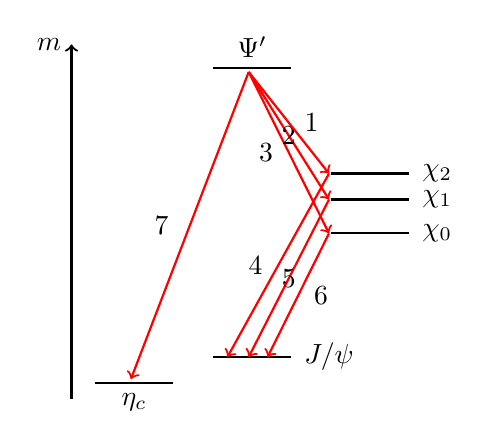
\begin{tikzpicture}[xscale=3,yscale=1]
      \draw[thick] (0,0) --++ (0.33,0) node[midway, below] {$\eta_c$};
      \draw[thick] (0.5,0.33) --++ (0.33,0) node[right=1pt] {$J/\psi$};
     \draw[thick] (1,1.9) --++ (0.33,0) node[right=1pt] {$\chi_0$}; 
      \draw[thick] (1,2.33) --++ (0.33,0) node[right=1pt] {$\chi_1$};
      \draw[thick] (1,2.66) --++ (0.33,0) node[right=1pt] {$\chi_2$};
      \draw[thick] (0.5,4) --++ (0.33,0) node[above,midway] {$\Psi'$};
   
    \draw[->,thick,red] (0.65,3.95) -> (0.1515,0.05) node[midway,black,left=4pt] {7};
    \draw[->,thick,red] (0.65,3.95) -> (0.99,1.9) node[midway,black,left=2pt] {3};
    \draw[->,thick,red] (0.65,3.95) -> (0.99,2.33) node[midway,black] {2};
    \draw[->,thick,red] (0.65,3.95) -> (0.99,2.66) node[midway,black,right=2pt] {1};

    \draw[->,thick,red] (0.99,1.9) -> (0.73,0.33) node[midway,black,right=2pt] {6};
     \draw[->,thick,red] (0.99,2.33) -> (0.65,0.33) node[midway,black] {5};
      \draw[->,thick,red] (0.99,2.66) -> (0.56,0.33) node[midway,black,left=2pt] {4};

      
     \draw[->,thick] (-0.1,-0.2) --++ (0,4.5) node[left] {$m$};  

   % \draw[<-,thick,blue!90!black] (0.2,0) --++ (0,3.5) node[above=40pt,right,midway,scale=0.8] {$E=h\cdot f_3$};
   % \draw[<-,thick,green!90!blue] (0.4,0) --++ (0,3) node[above=27pt,right,midway,scale=0.8] {$E=h\cdot f_2$};
   % \draw[<-,thick,red] (0.6,0) --++ (0,2) node[right,midway,scale=0.8] {$E=h\cdot f_1$};

    
\end{tikzpicture}
\end{minipage} %\pause
\underline{HOWEVER:}\\
\begin{itemize}
\item Spectrum of $c\Bar{c}$ is very easy to model
\item \textcolor{red}{Spectra of hadrons are often complicated and unknown} %\pause
\item[\ding{43}]Our task this afternoon!
\end{itemize}
\end{frame}
\subsection{}
%%%%%%%%%%%%%%%%%%%%%%%%%%%%%%%%%%%%%%%%%%%%%%%%%%%%%%%%%%%%%%%%%%%%%%%%%%%%%%%%%%%%%%%%%%%%%%
\begin{frame}{The most important thing}
    \begin{itemize}
        \item Hadrons (baryons and mesons) can be built from quarks
        \item Hadrons are colour-neutral, quarks carry colour
        \item Quarks can never be observed alone
        \item The top quark is too heavy to form hadrons
        \item $\Omega_c^0$ (ssc) and $\Xi_c^+$ (usc)
        \item Hadrons can be excited $\rightarrow$ Mass differences 
        \item [\ding{43}] We can learn about the nature of matter through spectroscopy!
    \end{itemize}
 \end{frame}
%%%%%%%%%%%%%%%%%%%%%%%%%%%%%%%%%%%%%%%%%%%%%%%%%%%%%%%%%%%%%%%%%%%%%%%%%%%%%%%%%%%%%%%%%%%%%%
\section{}
\begin{frame}{References}\footnotesize
    \begin{itemize}
    \item[-] Janzen, A. Ultraschnelle Elektronenbeugung an Oberflächen (2009)
    \item[-] Königsmann, K. Radiative decays in the $\Psi$ family. Physics Reports 139(5)(1986), 243-291.
    \item[-] Workman, R.L. et al. (PDG), Prog. Theor. Exp. Phys. (2022), 219
\item[-] schaette.de. \url{schaette.de/ratgeber/tiergesundheit/rinder/rinder-was-koennen-wir-fuer-abwehrstarke-kaelber-tun}
\item[-] meinhaushalt.at (2009). \url{meinhaushalt.at/4182-zunge-schalen-kochen/#}
\item[-] Airbus. \url{aircraft.airbus.com/en/aircraft/a320/a321xlr#images}
\item[-] Hegelrast 2019. CC BY-SA \url{https://commons.wikimedia.org/wiki/File:Coloured_flames_of_methanol_solutions_of_metal_salts_and_compounds.jpg} 


    \end{itemize}
\end{frame}
%%%%%%%%%%%%%%%%%%%%%%%%%%%%%%%%%%%%%%%%%%%%%%%%%%%%%%%%%%%%%%%%%%%%%%%%%%%%%%%%%%%%%%%%%%%%%%

\appendix


\subsection{schaette.de $|$ meinhaushalt.at}
\begin{frame}
\begin{minipage}{0.6\textwidth}
\includegraphics[width=\textwidth]{Figures Lecture on Hadrons/Hadron_with_pictures.png}
\end{minipage}
\begin{minipage}{0.38\textwidth}
The spectra of most hadrons are complicated and difficult to model.
\end{minipage}

\end{frame}
\subsection{}
\end{document}